\ifx\boi\undefined\ifx\problemname\undefined
\providecommand\sampleinputname{}
\providecommand\sampleoutputname{}
\documentclass[swedish]{templates/boi}
\problemlanguage{.sv}
\fi
\newcommand{\practicesession}{Övningssession}
\newcommand{\dayone}{Dag 1}
\newcommand{\daytwo}{Dag 2}
\newcommand{\boi}{Baltic Olympiad in Informatics}
\newcommand{\contestdates}{27 april - 1 maj, 2018}
\newcommand{\licensingtext}{Detta problem är licensierat enligt CC BY-SA 4.0.}
\newcommand{\problem}{Problem}
\newcommand{\inputsection}{Indata}
\newcommand{\outputsection}{Utdata}
\newcommand{\interactivity}{Interaktivitet}
\newcommand{\grading}{Bedömning}
\newcommand{\scoring}{Poängsättning}
\newcommand{\constraints}{Begränsningar}
\renewcommand{\sampleinputname}{Exempel-indata}
\renewcommand{\sampleoutputname}{Exempel-utdata}
\newcommand{\sampleexplanation}[1]{Förklaring till Exempel #1}
\newcommand{\sampleexplanations}{Förklaring till exemplen}
\newcommand{\timelimit}{Tidsgräns}
\newcommand{\memorylimit}{Minnesgräns}
\newcommand{\seconds}{s}
\newcommand{\megabytes}{MB}
\newcommand{\group}{Grupp}
\newcommand{\points}{Poäng}
\newcommand{\limitsname}{Gränser}
\newcommand{\additionalconstraints}{Övriga begränsningar}
\newcommand{\testgroups}{
Your solution will be tested on a set of test groups, each worth a number of points. Each test group contains
a set of test cases. To get the points for a test group you need to solve all test cases in the test group. Your
final score will be the maximum score of a single submission.

Din lösning kommer att testas på en uppsättning testgrupper, var och en värd en viss poäng.
Varje testgrupp innehåller flera testfall. 
För att få poäng för en testgrupp måste du klara alla testfallen i gruppen.
Din slutgiltiga poäng på problemet kommer att vara den maximala poängen av en enda submission.
}

\fi
\def\version{jury-1}
\problemname{Vägar}
En {\em graf} är en matematisk struktur som består av en uppsättning {\em noder}, och en uppsättning {\em bågar}, där varje båge sammanbinder två noder. Ett exempel på en graf med $4$ noder och $3$ bågar visas i exempelförklaringen nedan.

En {\em väg} i grafen definieras som en ordnad lista med $2$ eller fler noder, där det finns en båge mellan den första och andra noden i listan, mellan den andra och tredje, o.s.v. genom hela listan. Vi är bara intresserade av {\em enkla vägar} som inte innehåller samma nod flera gånger. Notera att listan är ordnad; exempelvis betraktas ``\texttt{5-6-7}'', ``\texttt{5-7-6}'' och ``\texttt{7-6-5}'' som olika vägar.

I den här uppgiften har varje nod i grafen en av $K$ färger. Uppgiften är att hitta antalet möjliga (enkla) vägar i vilka alla noder har olika färg.

\section*{\inputsection}
Första raden innehåller tre heltal: $N$ (antalet noder), $M$ (antalet bågar), och $K$ (antalet olika färger).

Andra raden innehåller $N$ heltal mellan $1$ och $K$ -- färgen på varje nod (första talet beskriver nod nummer $1$ och sista talet nod nummer $N$). 

Var och en av de följande $M$ raderna beskriver en båge och innehåller två heltal $a, b$ ($1 \le a, b \le N, a \neq b$) -- de två noderna som bågen sammanbinder. Det finns aldrig mer än en båge mellan samma två noder.

\section*{\outputsection}
Skriv ut ett heltal -- antalet vägar vars samtliga noder har olika färger. Antalet kommer alltid att vara lägre än $10^{18}$.

\section*{\constraints}
\testgroups

\noindent
\begin{tabular}{| l | l | l |}
\hline
\group & \points & \limitsname \\ \hline
1      & 23      & $1 \le N, M \le 100, 1 \le K \le 4$ \\ \hline
2      & 20      & $1 \le N, M \le 300\,000, 1 \le K \le 3$ \\ \hline
3      & 27      & $1 \le N, M \le 300\,000, 1 \le K \le 4$ \\ \hline
4      & 30      & $1 \le N, M \le 100\,000, 1 \le K \le 5$ \\ \hline
\end{tabular}

\section*{\sampleexplanation{1}}

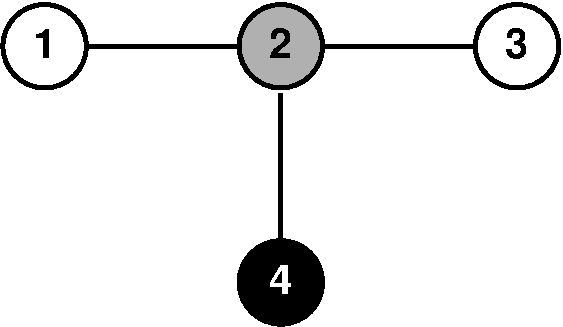
\includegraphics[width=5cm]{pathsfig.pdf}

Grafen i första exemplet visas i figuren, där varje nod har färgats vit (färg 1), grå (färg 2) eller svart (färg 3). Det finns 10 vägar vars noder har olika färger: ``\texttt{1-2}'', ``\texttt{2-1}'', ``\texttt{2-3}'', ``\texttt{3-2}'', ``\texttt{2-4}'', ``\texttt{4-2}'', ``\texttt{1-2-4}'', ``\texttt{4-2-1}'', ``\texttt{3-2-4}'' och ``\texttt{4-2-3}''.

Notera att ``\texttt{1}'' inte är en godkänd väg eftersom det är en ensam nod, och inte heller ``\texttt{1-2-3}'', eftersom den innehåller två noder med färg $1$.

